\documentclass[12pt, letterpaper]{article}

\usepackage{tikz}
\usepackage{amsmath}
\usepackage{geometry}
\usepackage{parskip}          % For better spacing between paragraphs
\usepackage{microtype}        % For better typography
\usepackage{titlesec}         % To customize section titles
\usepackage{setspace}         % For line spacing
\usepackage{fancyhdr}
\usepackage{hyperref}
\usepackage{microtype}
\usepackage[dvipsnames]{xcolor}
\usepackage{lmodern}
\usepackage{ulem}

\usepackage{tcolorbox}



\pagestyle{fancy}
\fancyfoot[L]{Problems of the Week - Solutions}
\fancyhead{}
\renewcommand{\headrulewidth}{0pt}

\setlength{\headheight}{15pt}

\hypersetup{
    colorlinks=true,
    linkcolor=blue,
    filecolor=magenta,      
    urlcolor=cyan,
    pdftitle={Problems of the Week, 3.2},
    pdfpagemode=FullScreen,
}

% \renewcommand{\headrulewidth}{0pt} 

\onehalfspacing

\titleformat{\section}{\large\bfseries}{\thesection}{1em}{}
\titlespacing*{\section}{0pt}{2em}{1em}

\title{\vspace{-2cm}Problems of the Week --- Évariste \\ Season 3 \\ Week 2 \\ Solutions}
\author{Taraash, Himanshu, Farhan, Rachit}
\date{\today}

\begin{document}
\maketitle

\section*{Intro}
Thank you for participating! These problems (especially Q2), were very challenging, but that doesn't mean they weren't nice, or fun to solve. I hope you had fun solving them! Q1 was from Putnam (only the first one though), so it may have misled you into thinking it was more complicated than it really was! Q2 was from this years SMMC (the \href{https://www.simonmarais.org/}{\color{orange} the Simon Marais mathematics competition}), which is indeed difficult, but once you have listed down a few numbers, the pattern should've been clear, though proving it would have taken a bit more. Q3 was from INMO, that's why it was probably kind of boring (they are kinda like that, but I never said it). Anyway! I hope you enjoyed solving these problems, feel free to reach us if you want to, hopefully this PDF will help you clear up anything you might've found confusing, and see you on the next (and last) set of the month.
\newpage

\section{Calculus}
For a positive integer $n$, let \(f_n(x) = \cos{(x)}\cos{(2x)}\cdots\cos{(nx)}\). Find the smallest $n$ such that \(|f_n^{''}(0)| > 2023\). {\color{gray}(A1, $84^{th}$ Putnam)}

\section*{Solution}
\colorbox{Dandelion}{Always try taking small, manageable value of $n$ to see wassup.}\\
Here, let's assume $n=3$, which gives us $f_3$, but to be more general, let us take \[
g(x)=\cos{(ax)}\cos{(bx)}\cos{(cx)}
\]
And just differentiate! 
\begin{align*}
    g^{'}(x) = &-a\cdot\sin(ax)\cos(bx)\cos(cx) \\
    &-b\cdot\cos(ax)\sin(bx)\cos(cx) \\
    &-c\cdot\cos(ax)\cos(bx)\sin(cx)
\end{align*}

Once more, and given we need to evaluate the double derivative at 0, we can knock off terms with a $\sin$ as $\sin(0)=0$, and $\cos$ vanishes too since $\cos(0)=1$. Which will leave us with \[
g^{''}(0) = -a^2 - b^2 - c^2
\]

Extrapolating to the general case, we get \[
f_n^{''}(0) = -1^2 -2^2 - 3^2 \cdots - n^2
\]

Which ofcourse simplifies to \[
f_n^{''}(0) = -\frac{n(n+1)(2n+1)}{6}
\]

Hence we have to solve for the smallest $n$ which satisfies
\[
\frac{n(n+1)(2n+1)}{6} > 2023
\]

Which gives us \colorbox{Turquoise}{$n=18$}.

\subsection*{Alternate Solution:}
I saw a lot of people doing this question in the way I'm about to describe, so, here:

\setlength{\jot}{6pt}
\begin{align*}  
f_n(x) = \prod_{i=1}^n\cos(ix) \\
\log{(f_n(x))} = \sum_{i=1}^{n}\log{(\cos{(ix)})}\\
\log{(f_n(x))}'=\frac{f_n'(x)}{f_n(x)}=-\sum_{i=1}^ni\cdot\frac{\sin(ix)}{\cos{(ix)}}\\
f_n'(x) = \left[-\sum_{i=1}^ni\cdot\tan{(ix)}\right]f_n(x)\\
f_n''(x) = \left[-\sum_{i=1}^ni\cdot\tan{(ix)}\right]f_n'(x) + \left[-\sum_{i=1}^ni\cdot (i\cdot\sec^2{(ix)})\right]f_n(x)\\
\texttt{At $x=0$}\\
\texttt{$f_n(0)=1$ since $\cos{0}=1$ and $f'_n(0)=0$ since $\tan{0}=0$ and $\sec{0}=1$}\\
f''_n(0)=-\sum_{i=1}^ni^2\\
\texttt{Hence we just need to solve}\\
|f''_n(0)|\rightarrow\frac{n(n+1)(2n+1)}{6} > 2024
\end{align*}
By just plugging and checking, we see $n=18$ is the least $n$ that satisfies the inequality.

\newpage

\section{Algebra} 
We define a positive integer $n$ as \textit{tripairable} if the set $\{1,2,\cdots,n\}$ can be partitioned into disjoint pairs such that the sum of the two elements in each pair is a power of 3. For example, 6 is tripairable because \(\{1,2,3,4,5,6\} = \{1,2\} \cup \{3,6\} \cup \{4,5\} \) and \[1+2=3^1, \quad 3+6=3^2 \quad and \quad 4+5=3^2\] are all powers of 3.
How many positive integers less than 2024 are tripairable? {\color{gray} (A2, SMMC 2024)}\\
Note that the official question had "less than or \underline{\textit{equal to}}
2024", I accidentally missed out on the "equal to", which resulted in one less (2024 is tripairable). This also unexpectedly became a good way to see who cheated!

\section*{Solution}
A fun one! \\
\colorbox{Dandelion}{Get your hands dirty! Take multiple values of $n$ and see if you can spot a pattern.}
{(\textit{Note that all tripairables will be even})}\\
If $k$ is tripairable, assume $n$ ($>k$) \[
\{1,2,3,\cdots,k,k+1,\cdots,n\}
\]
$k_{max}$ will be tripairable if 
\begin{align*}
    (k)+(1) = &3^a \\
    (k-1)+(2)=&3^a\\
    \textit{And so forth}
\end{align*}
For $n_{min}$ to be tripairable, we must have
\begin{align*}
    (n)+(k+1) = &3^{a+1} \\
    (n-1)+(k+2)=&3^{a+1}\\
    \textit{And so forth}
\end{align*}
If $k+1=3^a$, our next minimum tripairable number must be $n=3^{a-1}-3^a=2\cdot3^a$

Hence, no number in the interval $[3^a, 2*3^{a})$ is tripairable.\\\\
\textbf{\color{red}Lemma 1.} \textit{Proof done above.}\\
\colorbox{Gray}{Every number of the form $2*3^a$ for any non-negative integer $a$ is tripairable.}\\\\
\textbf{\color{green!70}Lemma 2.} \textit{Lemma 3 captures this case.}\\
\colorbox{Gray}{Every number of the form $3^a-1$ for any non-negative integer $a$ is tripairable.}\\\\
\textbf{\color{blue}Lemma 3.} \textit{Try yourself, take a look at the \href{https://www.simonmarais.org/uploads/8/2/3/5/82358688/smmc_2024_solutions.pdf}{\color{orange}official solution.}}\\
\colorbox{Gray}{Numbers of the form $2*3^a \texttt{ + previous tripairable numbers}$ are one too.}
\\\\
For any $a$, let's consider the interval $2*3^a\leq n\leq3^{a+1}-1$.
Let's now go over the values of $a$:
\begin{align}
    a=0 \implies& n={\color{red}2} \\
    a=1 \implies& n={\color{red}6} \And {\color{blue}6+2} \\
    a=2 \implies& n={\color{red}18} \And {\color{blue}18+2,18+6,18+6+2}
\end{align}

Hence, for any $a$, we have $n_{max} = 3^{a+1}-1$ and $n_{min}=2*3^a$ with a total of $2^a$ tripairable numbers between \textit{(inclusive)}. (you could show this inductively.)\\
As a corollary, we get $2^a-1$ tripairable numbers less than or equal to $3^a$.

The maximum value $a$ can take is 6, when $n_{max}$ exceeds the limit given (2024).

When $a=6$
\begin{align}
n_{max}=&2186 \\
n_{min} =& 1458 \\
n_{max, a=5} =& 728\\
n_{min, a=5} =& 486\\
1458+486+x<&2024 \implies x < 80
\end{align}

Finally:
\begin{align*}
    a=0 &\implies 2^0 \\
    a=1 &\implies 2^1 \\
    a=2 &\implies 2^2 \\
    a=3 &\implies 2^3 \\
    a=4 &\implies 2^4 \\
    a=5 &\implies 2^5 \\
    a=6 &\implies \underbrace{1+2^0+2^1+2^2+2^3+2^4}_{\text{adding till }a=4}+\underbrace{1+2^0+2^1+2^2+\overset{80 \text{ was over counted in set }a=3}{2^3-1}}_{\text{elements of }a=5\text{ taken only till }a=3\text{ ($n_{max,a=3}=80$)}}
\end{align*}
A little (lot) info about what we just did, we know that all tripairables are of the form $2*3^a$ + previous tripairable numbers, for $a=6$, we start with 1458, and end with 2187, which is $1458+728$, we can safely add all tripairables from the "set" $a\leq4$ as $n_{max, a=4}=242$ and $1458+242$ is within bounds, it gets tricky when $a=5$, we know tripairables in "set" $a=5$ are of the form $486, 486+\texttt{previous tripairables}$, so we get something like $1458+486+\texttt{pre}=1944+\text{pre}<2024$, so the maximum we can add is just smaller than $2024-1944=80$, take a look at all the tripairable I have listed down below; for $a=6$, we at maximum get 1458+566, 1458+486+80, which leads to a total of $$\underbrace{(2^6-1)}_{\text{till }a=5}+\overset{(a=6)}{(\underbrace{2^6}_{\text{if we had no limit}}-\underbrace{17}_{\text{but we do, so subtracting the extras}})}$$

Summing these up, we get the total number of tripairable integers less than 2024 as \colorbox{Apricot}{110}.

(I know this might be difficult to understand, the \href{https://www.simonmarais.org/uploads/8/2/3/5/82358688/smmc_2024_solutions.pdf}{\color{orange}official SMMC solution} is short and crisp, but confusing (remember that I made that typo in writing down the question, so the answer to the question written above is 110, while that of the SMMC 2024/A2 is 111), if you need further help, let me know; I may make a video explaining it.)

\subsection{All tripairables:}
${\color{teal}2}, {\color{RubineRed}6, 8}, {\color{teal}18, 20, 24, 26}, {\color{RubineRed}54, 56, 60, 62, 72, 74, 78, 80},$ \\${\color{teal}162, 164, 168, 170, 180, 182, 186, 188, 216, 218, 222, 224, 234, 236, 240, 242}$\\$\color{RubineRed}486, 488, 492, 494, 504, 506, 510, 512, 540, 542, 546, 548, 558, 560, 564, 566,$\\$
{\color{RubineRed}648, 650, 654, 656, 666, 668, 672, 674, 702, 704, 708, 710, 720, 722, 726, 728}$\\
${\color{teal}1458, 1460, 1464, 1466, 1476, 1478, 1482, 1484, 1512, 1514, 1518, 1520, 1530, 1532, 1536, 1538,}$\\$\color{teal}
1620, 1622, 1626, 1628, 1638, 1640, 1644, 1646, 1674, 1676, 1680, 1682, 1692, 1694, 1698, 1700,$\\$\color{teal}
1944, 1946, 1950, 1952, 1962, 1964, 1968, 1970, 1998, 2000, 2004, 2006, 2016, 2018, 2022$\\{\color{teal}\sout{\text{$
2024, 2106, 2108, 2112, 2114, 2124, 2126, 2130, 2132, 2160, 2162, 2166, 2168, 2178, 2180, 2184, 2186$}}}
\newpage


\section{Counting}
All the squares of a \( 2024 \times 2024 \) board are coloured white. In one move, you can select one row or column whose every square is white, choose exactly 1000 squares in this row or column, and colour all of them red. Find the maximum number of squares that you can colour red in a finite number of moves. {\color{gray} (Q2, $38^{th}$ INMO)}

\section*{Solution}
\colorbox{Dandelion}{Try to take the simplest case here. We will also generalize it to increase our flexibility.}\\\\
Assume our board is $n \times n$ and after every turn we color $k$ squares red. (with $k \leq n$)\\
As I said, take the simplest case. Take all $k$ columns/rows to be consecutive. Start by selecting all ($n$) columns, we are left we $n-k$ \emph{good} rows, select and color those. We claim that is the maximum we can do (which is $n\cdot k$ for the columns and $(n-k)\cdot k$ for the rows, which, after addition leaves us with $k\cdot (2n-k)$ tiles coloured.)

\begin{center}
    
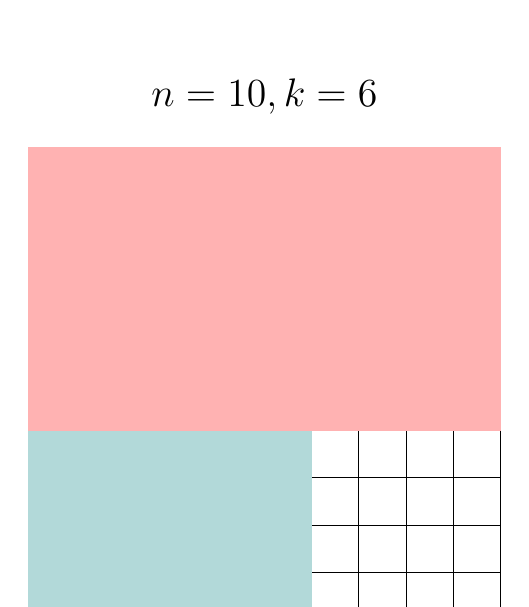
\begin{tikzpicture}[scale=0.6]
    \foreach \x in {0, 1, ..., 9} {
        \foreach \y in {0, 1, ..., 9} {
            \draw (\x, \y) rectangle (\x+1, \y+1);
        }
    }

    \foreach \x in {0, 1, ..., 9} {
        \foreach \y in {4, 5, 6, 7, 8, 9} {
            \fill[red!30] (\x, \y) rectangle (\x+1, \y+1);
        }
    }

    \foreach \x in {0, 1, 2, 3, 4, 5} {
        \foreach \y in {0, 1, 2, 3} {
            \fill[teal!30] (\x, \y) rectangle (\x+1, \y+1);
        }
    }

    \node[above] at (5, 10.5) {\Large $n=10, k=6$};
\end{tikzpicture}
\end{center}
Note that I'm using different colors for rows and columns for the sake of simplicity, but ofcourse we are using a single color in reality.

To prove this, consider choosing any row or column and coloring $k$ of it's tiles. After doing so, we leave $k+1$ rows and columns unusable as they have a red tile.
\begin{center}
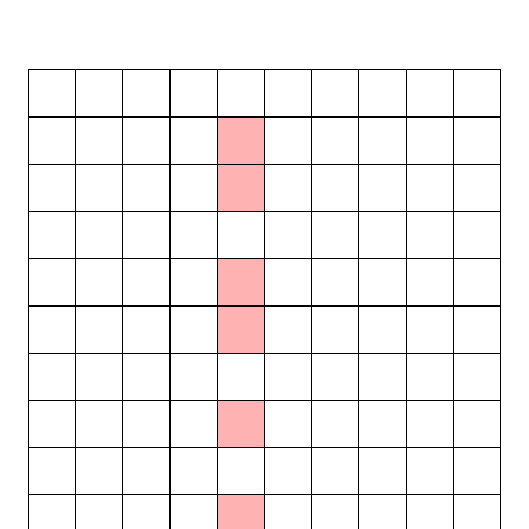
\begin{tikzpicture}[scale=0.6]
 \foreach \y in {0,2,4,5,7,8} {
            \fill[red!30] (4, \y) rectangle (5, \y+1);
        }
    \foreach \x in {0, 1, ..., 9} {
        \foreach \y in {0, 1, ..., 9} {
            \draw (\x, \y) rectangle (\x+1, \y+1);
        }
    }

       
\end{tikzpicture}
\end{center}

Each subsequent move necessarily reduces our possible options of choosing a row/column by 1 (consider choosing the adjacent column in our diagram, which is the least \emph{destructive} move).
\begin{center}
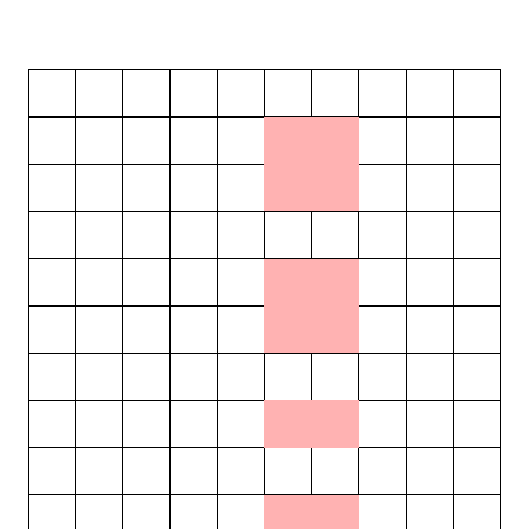
\begin{tikzpicture}[scale=0.6]
    \foreach \x in {0, 1, ..., 9} {
        \foreach \y in {0, 1, ..., 9} {
            \draw (\x, \y) rectangle (\x+1, \y+1);
        }
    }

    \foreach \x in {5,6} {
        \foreach \y in {0,2,4,5,7,8} {
            \fill[red!30] (\x, \y) rectangle (\x+1, \y+1);
        }
        }
\end{tikzpicture}
\end{center}

Since our number of colored tiles is directly proportional to the number of moves we play, we have to maximize our number of moves, which means playing the least destructive move each turn (which we know is 1, that is, after each move following the first, we have a move that only reduces our list of next possible moves by 1.)\\\\ An interesting case may be when we've exhausted our columns and now run to the rows:

\begin{center}
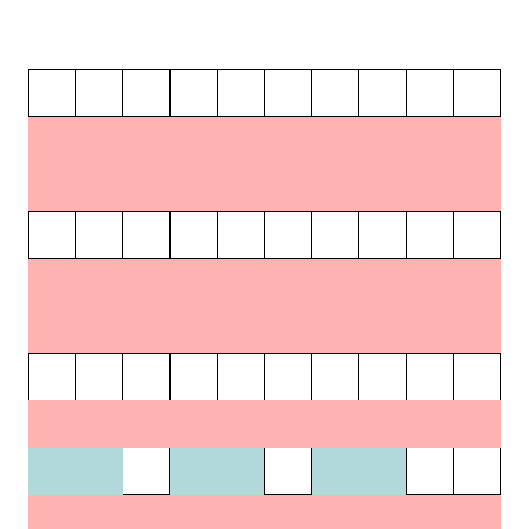
\begin{tikzpicture}[scale=0.6]
    \foreach \x in {0, 1, ..., 9} {
        \foreach \y in {0, 1, ..., 9} {
            \draw (\x, \y) rectangle (\x+1, \y+1);
        }
    }

    \foreach \x in {0,1, ..., 9} {
        \foreach \y in {0,2,4,5,7,8} {
            \fill[red!30] (\x, \y) rectangle (\x+1, \y+1);
        }
    }
    
    \foreach \x in {0,1,3,4,6,7} {
        \foreach \y in {1} {
            \fill[teal!30] (\x, \y) rectangle (\x+1, \y+1);
        }
    }
\end{tikzpicture}
\end{center}

\textit{Since we've exhausted our columns, we are only left with rows, and after each move, we are left with one less option, as was needed.}

Finally, we can, at maximum, choose $n$ columns and $n-k$ rows, which totals to a maximum of $k\cdot (n + n - k)$ red tiles.

Putting $n=2024$ and $k=1000$, we get our answer: \[
1000 \times (2*2024 - 1000) = \colorbox{Turquoise}{3048000}.
\]

\newpage

{\color{RubineRed} \rule{\linewidth}{0.5mm}}
\headrule{\color{RubineRed}  NOTES}
\vspace{20pt}
\begin{enumerate} 
\item  If I made any mistake, either in solving the problem, or just a typo (which is not unlikely), please let me know so I can fix it.
\item I have been pretty thorough here (I hope!), if you don't get something, please message us and we'll try to be even clearer.
\item Your solution can be different! My way of solving is likely different than yours, so if you've come up with a different solution, and if I like it, I may post it on telegram, or eventually in this doc.
\item That's it! Hope you had fun, and see you next week?
\end{enumerate}

\vspace{50pt}
\begin{center}

\begin{tikzpicture}
\color{ForestGreen}
  \draw[scale=0.5,domain=0:360,smooth,variable=\t] plot(\t:{sin(10*\t)});
\end{tikzpicture}
\end{center}

\end{document}
